% Author: Izaak Neutelings (October 2020)
\documentclass[border=3pt,tikz]{standalone}
\usepackage{physics}
\usepackage{tikz}
\usepackage[outline]{contour} % glow around text
\usetikzlibrary{calc}
\usetikzlibrary{angles,quotes} % for pic
\tikzset{>=latex} % for LaTeX arrow head
\contourlength{2pt}
\usetikzlibrary{patterns,snakes}
\usetikzlibrary{decorations.pathmorphing} % for decorate random steps

\colorlet{xcol}{blue!70!black}
\colorlet{vcol}{green!60!black}
\colorlet{myred}{red!65!black}
\colorlet{acol}{red!50!blue!80!black!80}
\tikzstyle{mass}=[line width=0.6,red!30!black,fill=red!40!black!10,rounded corners=1,
                  top color=red!40!black!20,bottom color=red!40!black!10,shading angle=20]
\tikzstyle{rvec}=[->,xcol,very thick,line cap=round]
\tikzstyle{pvec}=[->,myred,very thick,line cap=round]
\tikzstyle{velocity}=[->,vcol,very thick,line cap=round]

\tikzset{
  pics/collision/.style={
    code={
      \draw[line width=0.5*#1,orange,fill=yellow]
        (0:0.20*#1) -- (30:0.06*#1) -- (50:0.25*#1) -- (80:0.10*#1) -- (105:0.32*#1) --
        (140:0.08*#1) -- (170:0.25*#1) -- (190:0.08*#1) -- (220:0.25*#1) --
        (250:0.08*#1) -- (270:0.24*#1) -- (300:0.08*#1) -- (320:0.25*#1) -- (340:0.09*#1) -- cycle;
  }},
  pics/collision/.default=1,
}


\begin{document}


% CENTER OF MASS 2D
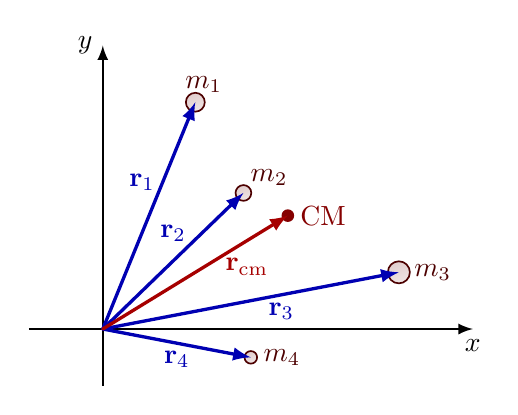
\begin{tikzpicture}
  \def\xmax{4.7} % max x axis
  \def\ymax{3.6} % max y axis
  \coordinate (O) at (0,0);
  \coordinate (M1) at (0.25*\xmax, 0.80*\ymax);
  \coordinate (M2) at (0.38*\xmax, 0.48*\ymax);
  \coordinate (M3) at (0.80*\xmax, 0.20*\ymax);
  \coordinate (M4) at (0.40*\xmax,-0.1*\ymax);
  \coordinate (CM) at (0.50*\xmax, 0.4*\ymax);
  \draw[->,thick] (0,-0.2*\ymax) -- (0,\ymax) node[left] {$y$};
  \draw[->,thick] (-0.2*\xmax,0) -- (\xmax,0) coordinate (X) node[below] {$x$};
  \draw[mass] (M1) circle(0.12) node[right=3,above=0] {$m_1$};
  \draw[mass] (M2) circle(0.10) node[above right=-1] {$m_2$};
  \draw[mass] (M3) circle(0.14) node[right=2] {$m_3$};
  \draw[mass] (M4) circle(0.08) node[right=1] {$m_4$};
  \fill[myred!80!black] (CM) circle(0.08) node[right=1] {CM};
  \draw[rvec] (O) -- (M1) node[midway,above=12,left=-6] {$\vb{r}_1$};
  \draw[rvec] (O) -- (M2) node[midway,right=0,above=3] {$\vb{r}_2$};
  \draw[rvec] (O) -- (M3) node[midway,right=11,below=-3] {$\vb{r}_3$};
  \draw[rvec] (O) -- (M4) node[midway,below=-1] {$\vb{r}_4$};
  \draw[rvec,myred] (O) -- (CM) node[midway,above=2,right=7] {$\vb{r}_\mathrm{cm}$};
\end{tikzpicture}


% CENTER OF MASS - bomb before
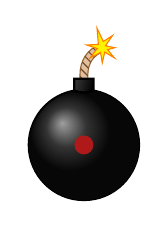
\begin{tikzpicture}
  \def\R{0.7}  % radius
  \def\h{0.15} % height fuse box
  \coordinate (O) at (0,0);
  \draw[thin,preaction={draw=brown!80!black,fill=brown!50},
        pattern color=brown!60!black,pattern=north west lines,draw=none,minimum width=0.1,minimum height=0.6]
    (0.05,\R+0.95*\h) --++ (0,0.3*\h) to[out=90,in=-160]++ (0.2,0.3) --++ (110:0.1) node[midway] (F) {}
    to[out=-160,in=90]++ ({-0.3+0.1*cos(70)},{-0.3-0.1*sin(70)}) --++ (0,-0.3*\h) -- cycle;
  \pic[scale=1] at (F) {collision={0.8}};
  \draw[thick,ball color=black] (O) circle(\R);
  \fill[thick,black!90,opacity=0.3] (O) circle(\R);
  \draw[thick,top color=black!80,bottom color=black,shading angle=75]
    (80:\R) |-++ ({-2*\R*sin(10)},\h) -- (100:\R) to[out=-20,in=-160] cycle;
  \fill[myred!90] (O) circle(0.12); %node[right=1] {\contour{black!20}{cm}};
\end{tikzpicture}


% CENTER OF MASS - bomb after
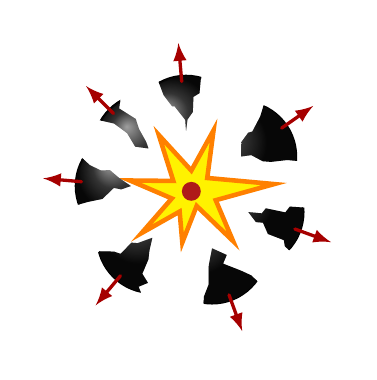
\begin{tikzpicture}
  \def\R{0.7} % radius
  \coordinate (O) at (0,0);
  \pic[scale=1,rotate=-100] at (O) {collision={3.3}};
  \fill[myred!90] (O) circle(0.12); %node[right=1] {\contour{black!20}{cm}};
  %\draw[thick,ball color=black] (O) circle(\R);
  \foreach \anga/\angb [evaluate={\ang=(\angb+\anga)/2;}] in {0/70,70/120,120/150,150/200,200/260,260/320,320/360}{
    \begin{scope}[shift={(\ang:1.1*\R)}]
      \clip[decorate,decoration={random steps,segment length=4pt,amplitude=2pt}]
        (\anga:1.8*\R) arc(\anga:\angb:1.8*\R) -- (0,0) -- cycle;
      \draw[thick,ball color=black] (0,0) circle(\R);
      \fill[thick,black!90,opacity=0.3] (0,0) circle(\R);
      \draw[pvec] (\ang:0.9*\R) --++ (\ang:0.7*\R);
    \end{scope}
  }
\end{tikzpicture}


% CENTER OF MASS - bomb after
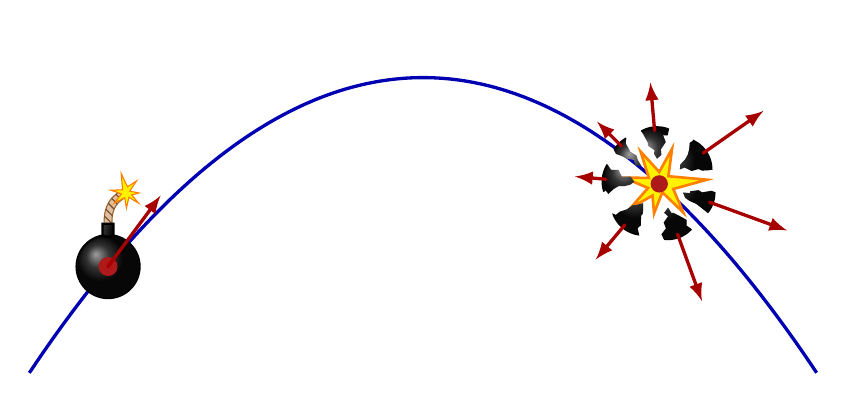
\begin{tikzpicture}
  \def\xmax{8}  % maximum x axis
  \def\A{0.15}  % amplitude of parabola
  \def\root{10} % root of parabola (intersection with x axis)
  \def\R{0.4}   % bomb radius
  \def\xi{1}    % bomb 0 x position
  \def\xa{8}    % bomb 1 x position
  \def\xb{9}    % bomb 2 x position
  \def\h{0.15}  % height fuse box
  \coordinate (O) at (0,0);
  \coordinate (B0) at (\xi,{\A*(\root-\xi)*\xi});
  \coordinate (B1) at (\xa,{\A*(\root-\xa)*\xa});
  \coordinate (B2) at (\xb,{\A*(\root-\xb)*\xb});
  \draw[xcol,very thick,variable=\x,samples=100,smooth,domain=0:\root]
    plot(\x,{\A*(\root-\x)*\x});
  
  % BOMB BEFORE
  \begin{scope}[shift={(B0)}]
    \draw[thin,preaction={draw=brown!80!black,fill=brown!50},
          pattern color=brown!60!black,pattern=north west lines,draw=none,minimum width=0.1,minimum height=0.6]
      (0.05,\R+0.95*\h) --++ (0,0.3*\h) to[out=90,in=-160]++ (0.2,0.3) --++ (110:0.1) node[midway] (F) {}
      to[out=-160,in=90]++ ({-0.3+0.1*cos(70)},{-0.3-0.1*sin(70)}) --++ (0,-0.3*\h) -- cycle;
    \pic[scale=1] at (F) {collision={0.8}};
    \draw[thick,ball color=black] (0,0) circle(\R);
    \fill[thick,black!90,opacity=0.3] (0,0) circle(\R);
    \draw[thick,top color=black!80,bottom color=black,shading angle=75]
      (80:\R) |-++ ({-2*\R*sin(10)},\h) -- (100:\R) to[out=-20,in=-160] cycle;
    \fill[myred!90] (0,0) circle(0.12); %node[right=1] {\contour{black!20}{cm}};
    \draw[pvec] (0,0) --++ ({atan(\A*(\root-\xi))}:2.8*\R);
  \end{scope}
  
  % BOMBS AFTER
  \pic[scale=1,rotate=-100] at (B1) {collision={1.9}};
  %\pic[scale=1,rotate=-100] at (B2) {collision={1.9}};
  \fill[myred!90] (B1) circle(0.11);
  %\fill[myred!90] (B2) circle(0.11);
  \foreach \anga/\angb [evaluate={\ang=(\angb+\anga)/2;}] in {0/70,70/120,120/150,150/200,200/260,260/320,320/360}{
    \begin{scope}[shift={($(B1)+(\ang:0.8*\R)$)}] % BOMB 1
      \clip[decorate,decoration={random steps,segment length=2pt,amplitude=1pt}]
        (\anga:4*\R) arc(\anga:\angb:4*\R) -- (0,0) -- cycle;
      \draw[thick,ball color=black] (0,0) circle(\R);
      \fill[thick,black!90,opacity=0.3] (0,0) circle(\R);
      \draw[pvec] (\ang:0.9*\R) --++ (\ang:{\R*(1.8+0.8*cos(\ang)-0.2*sin(\ang))});
    \end{scope}
    %\begin{scope}[shift={($(B2)+(\ang:2.5*\R)$)}] % BOMB 2
    %  \clip[decorate,decoration={random steps,segment length=5pt,amplitude=3pt}]
    %    (\anga:3*\R) arc(\anga:\angb:3*\R) -- (0,0) -- cycle;
    %  \draw[thick,ball color=black] (0,0) circle(\R);
    %  \fill[thick,black!90,opacity=0.3] (0,0) circle(\R);
    %  \draw[pvec] (\ang:0.9*\R) --++ (\ang:{\R*(1.6+0.8*cos(\ang)-0.5*sin(\ang))});
    %\end{scope}
  }
  
\end{tikzpicture}



% CENTER OF MASS 1D
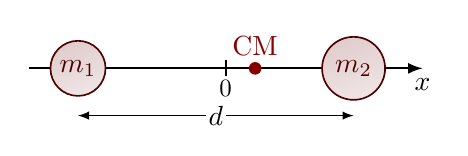
\begin{tikzpicture}
  \def\xmax{2.5} % max x axis
  \coordinate (O) at (0,0);
  \coordinate (M1) at (-0.75*\xmax,0);
  \coordinate (M2) at ( 0.65*\xmax,0);
  \coordinate (CM) at ( 0.15*\xmax,0);
  \draw[->,thick] (-\xmax,0) -- (\xmax,0) coordinate (X) node[below] {$x$};
  \draw[thick] (0,0.1) -- (0,-0.1) node[below=-1.8,scale=0.9] {0};
  \draw[<->] (M1)++(0,-0.6) --++ (1.4*\xmax,0) node[midway,fill=white,inner sep=1] {$d$};
  \draw[mass] (M1) circle(0.35) node {$m_1$};
  \draw[mass] (M2) circle(0.40) node {$m_2$};
  \fill[myred!80!black] (CM) circle(0.08) node[above=1] {CM};
\end{tikzpicture}


\end{document}